\documentclass[12pt]{extarticle}
\usepackage[utf8]{inputenc}
\usepackage[english]{babel}
\usepackage[a4paper, total={6in, 9in}]{geometry}
\usepackage{tikz-cd}
\usepackage{graphicx} 
 
\usepackage{amsthm, amssymb, amsmath, centernot}

\newcommand{\notimplies}{%
  \mathrel{{\ooalign{\hidewidth$\not\phantom{=}$\hidewidth\cr$\implies$}}}}
 
\renewcommand\qedsymbol{$\square$}
\newcommand{\cont}{$\boxtimes$}
\newcommand{\divides}{\mid}
\newcommand{\ndivides}{\centernot \mid}
\newcommand{\Z}{\mathbb{Z}}
\newcommand{\R}{\mathbb{R}}
\newcommand{\N}{\mathbb{N}}
\newcommand{\C}{\mathbb{C}}
\newcommand{\Zplus}{\mathbb{Z}^{+}}
\newcommand{\Primes}{\mathbb{P}}
\newcommand{\colim}[1]{\mathrm{colim}(#1)}
\newcommand{\Ob}[1]{\mathrm{Ob}(#1)}
\newcommand{\cat}[1]{\mathcal{#1}}
\newcommand{\id}{\mathrm{id}}
\newcommand{\Hom}[2]{\mathrm{Hom}\left( #1, #2 \right)}
\newcommand{\catHom}[3]{\mathrm{Hom}_{#1}\left( #2, #3 \right)}
\newcommand{\Top}{\mathbf{Top}}
\newcommand{\pTop}{\mathbf{Top}_{\bullet}}
\newcommand{\Set}{\mathbf{Set}}
\newcommand{\pSet}{\mathbf{Set}_\bullet}
\newcommand{\hTop}{\mathbf{hTop}}
\newcommand{\phTop}{\mathbf{hTop}_{\bullet}}
\renewcommand{\Im}[1]{\mathrm{Im}(#1)}
\newcommand{\homspace}[2]{\left< #1, #2 \right>}
\newcommand{\rp}{\mathbb{RP}}
\newcommand{\coker}[1]{\mathrm{coker}\: #1}

\renewcommand{\d}[1]{\: \mathrm{d}#1 \:}
\newcommand{\dn}[2]{\: \mathrm{d}^{#1} #2 \:}
\newcommand{\deriv}[2]{\frac{\d{#1}}{\d{#2}}}
\newcommand{\nderiv}[3]{\frac{\dn{#1}{#2}}{\d{#3^2}}}
\newcommand{\pderiv}[2]{\frac{\partial{#1}}{\partial{#2}}}
\newcommand{\parsq}[2]{\frac{\partial^2{#1}}{\partial{#2}^2}}

\theoremstyle{definition}
\newtheorem{theorem}{Theorem}[section]
\newtheorem{lemma}[theorem]{Lemma}
\newtheorem{proposition}[theorem]{Proposition}
\newtheorem{example}[theorem]{Example}
\newtheorem{corollary}[theorem]{Corollary}
\newtheorem{remark}{Remark}

\newenvironment{definition}[1][Definition:]{\begin{trivlist}
\item[\hskip \labelsep {\bfseries #1}]}{\end{trivlist}}


\newenvironment{lproof}{\begin{proof} \renewcommand{\qedsymbol}{}}{\end{proof}}
\renewcommand{\mod}[3]{\: #1 \equiv #2 \: mod \: #3 \:}
\newcommand{\nmod}[3]{\: #1 \centernot \equiv #2 \: mod \: #3 \:}
\newcommand{\ndiv}{\hspace{-4pt}\not \divides \hspace{2pt}}
\newcommand{\gen}[1]{\langle #1 \rangle}
\newcommand{\hook}{\hookrightarrow}
\newcommand{\Tor}[4]{\mathrm{Tor}^{#1}_{#2} \left( #3, #4 \right)}
\newcommand{\Ext}[4]{\mathrm{Ext}^{#1}_{#2} \left( #3, #4 \right)}

\tikzset{
    labl/.style={anchor=south, rotate=90, inner sep=.5mm}
}

\renewcommand{\bf}[1]{\mathbf{#1}}
\newcommand{\Class}[2]{\mathcal{C}^{#1} \left( #2 \right)}
\newcommand{\Res}[2]{\mathrm{Res}_{#1} \: #2}
\newcommand{\F}{\mathcal{F}}
\newcommand{\G}{\mathcal{G}}
\renewcommand{\O}{\mathcal{O}}
\newcommand{\supp}[1]{\mathrm{Supp}\left(#1\right)}

\title{Riemann Surfaces Midterm}
\author{Benjamin Church}
\date{December 17, 2018}


\begin{document}

\maketitle

\begin{remark}
Whenever I have the complex coordinate $z$, I will  denote the real coordinates by $x, y \in \R$ such that $z = x + iy$ and the derivatives $\partial = \partial_z$ and $\bar{\partial} = \partial_{\bar{z}}$.
\end{remark}

\section*{Problem 1}

Take six pairwise distinct points $a_1, a_2, a_3, a_4, a_4, a_5, a_6 \in \C$ and consider the equation,
\[ w^2 = \prod_{i = 1}^6 (x - a_i) \]
We wish to consider the compact Riemann surface $\hat{X}$ for this equation. I will assume, for convenience, that these points are all nonzero and not infinity although this assumption will not seriously affect my argument only remove degenerate cases.

\subsection*{(a)}

Consider two copies of the complex plane, called sheets, labeled (I) and (II). We give each sheet three branch cuts, $a_1$-$a_2$ and $a_3$-$a_4$ and $a_5$-$a_6$. 
Now we compactify each sheet by adding two points at infinity $\infty_{\mathrm{I}}$ and $\infty_{\mathrm{II}}$ to close them into a sphere with three holes. When we glue these two spheres with three holes along the boundaries of the holes we get a two holed torus $\hat{X}$ which is the unique orientable compact surface of genus $g = 2$.  
\begin{center}
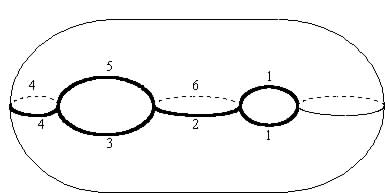
\includegraphics[scale=0.8]{TwoHoledTorus}
\end{center}
To make $\hat{X}$ a Riemann surface we need to choose a covering of $\hat{X}$ by holomorphic chars. For a point away from either $\infty$ and any branch point $a_i$ and any cut, we simply take a disk in the complex plane (I) or (II) with standard holomorphic coordinate. For a point near the cut, we take a half-disk on (I) which continues to a half-disk on (II) across the cut. At either $\infty$ we take the holomorphic coordinate $z = \zeta^{-1}$. At a branch point $a_i$ we take the holomorphic coordinate $z = a_i + \zeta^2$ where the double cover of the disk about $a_i$ by $\zeta^2$ is taken to be injective by sending the first covering to sheet (I) and the second covering to sheet (II). 
We need to show that $w$ is well-defined and meromorphic on $\hat{X}$. Away from branch points and infinities $w$ is a holomorphic function on $\C$ and thus on the holomorphic coordinate disks. Now we need to check the branch points. Near $z = a_i$ we have the holomorphic coordinate $z = \zeta^2 + a_i$ and thus,
\[ w(\zeta) = \pm \sqrt{\prod_{j = 1}^6 (\zeta^2 + a_i - a_j)} = \zeta \sqrt{\prod_{j \neq i}^6 (\zeta^2 + a_i - a_j)} \]
which is holomorphic on the $\zeta$ coordinate chart with a simple zero at $\zeta \to 0$ i.e. $z = a_i$. Next, near $z = \infty_{\mathrm{I}}$ we have the coordinate chart $z = \frac{1}{\zeta}$ and thus,
\[ w(\zeta) = \pm \sqrt{\prod_{j = 1}^6 (\zeta^{-1} - a_j)} = \zeta^{-3} \sqrt{\prod_{j = 1}^6 (1 - a_j \zeta)} \]
which has a triple pole at each $\infty$. I should remark that $\pm$ is shorthand notation for the fact that as $\zeta$ passes the negative imaginary axis we transition from (I) to (II) meaning that $w$ changes sign. This negative sign allows the manipulation $\pm \sqrt{\zeta^2} = \zeta$ since the sign information that would usually be lost in the choice of square root is preserved by the $\pm$ on different sheets. 

\subsection*{(b)}

We define two holomorphic forms on $\hat{X}$,
\begin{align*}
\omega_1 & = \frac{\d{z}}{w} = 
\begin{cases}
\frac{\d{z}}{\sqrt{\prod_{i = 1}^6 (z - a_i)}} &  z \in \mathrm{(I)}
\\
- \frac{\d{z}}{\sqrt{\prod_{i = 1}^6 (z - a_i)}} & z \in \mathrm{(II)}
\end{cases}
\\
\omega_2 & = \frac{z \d{z}}{w} = 
\begin{cases}
\frac{z \d{z}}{\sqrt{\prod_{i = 1}^6 (z - a_i)}} & z \in \mathrm{(I)}
\\
- \frac{z \d{z}}{\sqrt{\prod_{i = 1}^6 (z - a_i)}} & z \in \mathrm{(II)}
\end{cases}
\end{align*}
We need to check that these forms are holomorphic when expressed in terms of the local holomorphic variables on coordinate charts. At the branch point $a_i$, in terms of the local holomorphic coordinate $z = \zeta^2 + a_i$ we express the forms,
\begin{align*}
\omega_1 = \frac{\d{z}}{w} & = \pm \frac{\zeta \d{\zeta}}{\sqrt{\prod_{j = 1}^6 (\zeta^2 + a_i - a_j) }} = \frac{\d{\zeta}}{\sqrt{\prod_{j \neq i}^6 (\zeta^2 + a_i - a_j) }}
\\
\omega_2 = \frac{z \d{z}}{w} & = \pm \frac{(\zeta^2 + a_i) \zeta \d{\zeta}}{\sqrt{\prod_{j = 1}^6 (\zeta^2 + a_i - a_j) }} = \frac{(\zeta^2 + a_i) \d{\zeta}}{\sqrt{\prod_{j \neq i}^6 (\zeta^2 + a_i - a_j) }}
\end{align*}
which are well-defined and nonzero in the limit $\zeta \to 0$. Next, at each $\infty$ with local holomorphic coordinate $z = \zeta^{-1}$ the forms are,
\begin{align*}
\omega_1 = \frac{\d{z}}{w} & = - \frac{\zeta^{-2} \d{\zeta}}{\sqrt{\prod_{j = 1}^6 (\zeta^{-1} - a_j) }} = - \frac{\zeta^{-2} \d{\zeta}}{\zeta^{-3} \sqrt{\prod_{j = 1}^6 (1 - a_j \zeta) }} = - \frac{\zeta \d{\zeta}}{\sqrt{\prod_{j = 1}^6 (1 - a_j \zeta)}} 
\\
\omega_2 = \frac{z\d{z}}{w} & = - \frac{\zeta^{-3} \d{\zeta}}{\sqrt{\prod_{j = 1}^6 (\zeta^{-1} - a_j) }} = - \frac{\zeta^{-3} \d{\zeta}}{\zeta^{-3} \sqrt{\prod_{j = 1}^6 (1 - a_j \zeta) }} = - \frac{\d{\zeta}}{\sqrt{\prod_{j = 1}^6 (1 - a_j \zeta)}} 
\end{align*}
Both forms are well-defined and holomorphic in the limit $\zeta \to 0$. Furthermore, we see that $\omega_1$ has a simple zero at each $\infty$ and $\omega_2$ is nonzero near $\infty$. Therefore, $\omega_1$ and $\omega_2$ cannot be linearly dependent $(1,0)$-forms since they have different pole structures and are nonzero. Therefore, neither can be a multiple of the other. 
\bigskip\\
The zeros of these forms are interesting. We have shown that $\omega_1$ has simple zeros at $z = \infty_{\mathrm{I}}$ and $z = \infty_{\mathrm{II}}$ while $\omega_2$ is nonzero at all branch points and each $\infty$ but clearly has simple zeros at $z = 0_{\mathrm{I}}$ and $z = 0_{\mathrm{II}}$. We should expect this because as holomorphic $(1,0)$-forms, $\omega_1$ and $\omega_2$ are holomorphic sections of the canonical bundle $K_X$ and thus (since holomorphic forms have no poles) the number of zeros of each must equal $c_1(K_X) = - \chi(\hat{X}) = 2 g - 2 = 2$ where $g = 2$ is the genus of our Riemann surface.   

\subsection*{(c)}

Consider the form, 
\[ \omega_{a_i} =  \frac{\omega_1}{z - a_i} \]
I need to check that $\omega_{a_i}$ is meromorphic with exactly a double pole at $a_i$. First, near each $\infty$, in the local holomorphic coordinate $z = \zeta^{-1}$ we have,
\[ \omega_{a_i} = - \frac{\zeta^{-2} \d{\zeta}}{\sqrt{\prod_{j = 1}^6 (\zeta^{-1} - a_j)}} \cdot \frac{1}{\zeta^{-1} - a_i} = - \frac{\zeta^2 \d{\zeta}}{\sqrt{\prod_{j = 1}^6 (1 - a_j \zeta)}} \cdot \frac{1}{1 - a_i \zeta} \] 
Therefore $\omega_{a_i}$ has a double pole at each $\infty$. Next, at a branch point $a_k$ for $k \neq i$ we write the form in terms of the local holomorphic coordinate $z = \zeta^2 + a_k$ as,
\[ \omega_{a_i} = \pm \frac{\zeta \d{\zeta}}{\sqrt{\prod_{j = 1}^6 (\zeta^2 + a_k - a_j)}} \cdot \frac{1}{\zeta^2 + a_k - a_i} = \frac{\d{\zeta}}{\sqrt{\prod_{j \neq k}^6 (\zeta^2 + a_k - a_j)}} \cdot \frac{1}{\zeta^2 + a_k - a_i}\]
which is holomorphic and nonzero as $\zeta \to \infty$ since $a_k \neq a_i$. Finally, near $a_i$ and again using the local holomorphic coordinate $z = \zeta^2 + a_i$ we find,
\[ \omega_{a_i} = \pm \frac{\zeta \d{\zeta}}{\sqrt{\prod_{j = 1}^6 (\zeta^2 + a_i - a_j)}} \cdot \frac{1}{\zeta^2} = \frac{\d{\zeta}}{\sqrt{\prod_{j \neq i}^6 (\zeta^2 + a_i - a_j)}} \cdot \frac{1}{\zeta^2} \]
which has a double pole at $\zeta = 0$ i.e. at $z = a_i$. 
\bigskip\\
The meromorphic $(1,0)$-form $\omega_{a_i}$ has two poles at $z = a_i$. As a meromorphic section of $K_X$ know that,
\[ \text{(\# of zeros of $\omega_{a_i}$)} - \text{(\# of poles of $\omega_{a_i}$)} = c_1(K_X) = 2g - 2 = 2 \]
so $\omega_{a_i}$ must have four poles. We have seen this is the case because $\omega_{a_i}$ has a double pole at $\infty_{\mathrm{I}}$ and a double pole at $\infty_{\mathrm{II}}$. 

\section*{Problem 2}

Let $X$ be a compact Riemann surface and $p, q \in X$ be distinct points. 

\subsection*{(a)}

First, let $U \subset X$ be a coordinate chart with a chart map $\varphi : U \to D \subset \C$ to a disk in the complex plane such that $p, q \in U$. Denote the holomorphic coordinate $\varphi^{-1} : D \to U$ on $U \subset X$ by $z$ and the images of $p$ and $q$ in $D$ by $P$ an $Q$. Now, define,
\[  g =  \chi(z) \log{\left( \frac{z - P}{z - Q} \right)} \quad \text{and} \quad \tilde{\omega}_{pq} = \partial \left( \chi(z) \log{\left( \frac{z - P}{z - Q} \right)} \right) \d{z} \] 
where $\chi$ is a bump function with support contained in $U = \varphi^{-1}(D)$ such that $\chi \equiv 1$ on some compact disk $B \subset D$ large enough that $P, Q \in B^\circ$. Since $\supp{\tilde{\omega}_{pq}} \subset U$ we can extend $\tilde{\omega}_{pq}$ to a form on $X$ by taking it zero outside $U$. Furthermore, since $\chi \equiv 1$ on $B \subset D$, in that smaller disk,
\[ \tilde{\omega}_{pq} =  \partial \left( \log{\left( \frac{z - P}{z - Q} \right)} \right) \d{z} = \left( \frac{1}{z - P} - \frac{1}{z - Q} \right) \d{z} \]
which is meromorphic with simple poles at $p$ and $q$ and residues $+1$ and $-1$ respectively.
Furthermore, $g$ is holomorphic on $B \setminus L$ where $L$ is the line segment connecting $P$ and $Q$ which we can choose as the branch cut of the logarithm. The logarithm remains well-defined when traversing a loop around both $P$ and $Q$ because both $\log{(z - P)}$ and $\log{(z - Q)}$  pick up a factor of $2 \pi i$ which cancel. Therefore, if we do not cross the branch cut $L$, the logarithm remains well-defined. Furthermore,
\[ \bar{\partial} \tilde{\omega}_{pq} = \partial \bar{\partial} \left( \chi(z) \log{\left( \frac{z - P}{z - Q} \right)} \right) \d{z} \wedge \d{\bar{z}} \]
I claim that $\eta = \bar{\partial} g$
can be extended to a smooth $(0,1)$-form on $X$. First, outside $B$ we know that $\eta$ is a smooth form because $g$ is smooth and then identically zero. Furthermore, $g$ is holomorphic on $B \setminus L$ so $\bar{\partial} g = 0$ on $B \setminus L$. Therefore, we can extend $\eta \equiv 0$ on all of $B$ since $L \subset B^\circ$ without affecting its smoothness outside $B$. Thus, $\eta$ is a smooth $(0, 1)$-form on $X$. Now consider the equation,
\[ \bar{\partial} \partial u = \bar{\partial} \tilde{\omega}_{pq} \]
where $\bar{\partial} \tilde{\omega}_{pq}$ is a smooth $(1,1)$-form because $\bar{\partial} \tilde{\omega}_{pq} = \partial \eta$ or because $\tilde{\omega}_{pq}$ is smooth outside $B$ and holomorphic inside $B \setminus \{P,Q\}$ so $\bar{\partial} \tilde{\omega}_{pq} = 0$ on $B \setminus \{P,Q\}$ and can be extended to zero on all of $B$. Furthermore,
I can write, 
\[ \bar{\partial} \tilde{\omega}_{pq} = \partial \bar{\partial} \left( \chi(z) \log{\left( \frac{z - P}{z - Q} \right)} \right) \d{z} \wedge \d{\bar{z}} = \d{\left\{ \bar{\partial} \left( \chi(z) \log{\left( \frac{z - P}{z - Q} \right)} \right) \d{\bar{z}} \right\}} = \d{\eta} \]
since both sides are zero on $B$ and are smooth outside $B$. Above, I have used the identify, $\d{(f \d{\bar{z}})} = \partial f \d{z} \wedge \d{\bar{z}} + \bar{\partial} f \d{\bar{z}} \wedge \d{\bar{z}} = \partial f \d{z} \wedge \d{\bar{z}}$. Therefore,
\[ \int_X \bar{\partial} \tilde{\omega}_{pq} = \int_X \d{\eta} = 0 \]
by Stokes theorem because $X$ has no boundary and $\eta$ is a smooth $(0,1)$-form. By the PDE existence theorem proven in class, this implies the existence of a smooth solution $u$ on $X$. Let $\psi = \partial u$ which is a smooth $(1,0)$-form. Then, we have shown,
\[ \bar{\partial} \psi = \bar{\partial} \tilde{\omega}_{pq} \]
Define $\omega_{pq} = \tilde{\omega}_{pq} - \psi$ which has simple poles at exactly $p$ and $q$ since $\tilde{\omega}_{pq}$ is meromorphic inside $\varphi^{-1}(B) \subset U$ with simple poles as $p$ and $q$ while $\psi$ is smooth everywhere. Furthermore,
\[ \bar{\partial} \omega_{pq} = \bar{\partial} \tilde{\omega}_{pq} - \bar{\partial} \psi = 0 \]
so $\omega_{pq}$ is holomorphic wherever it is smooth i.e. everywhere but its poles $p$ and $q$ so $\omega_{pq}$ is the desired meromorphic form.

\subsection*{(b)}

Now suppose that $p$ and $q$ no not lie in the same coordinate chart of $X$. Let $\{ U_\alpha \}$ be a covering of $X$ by holomorphic coordinate charts. Since $X$ is compact, we may choose this covering to include a finite number, $N$, charts. Let $G$ be the graph on $N$ vertices representing the charts with an edge between two vertices exactly when their corresponding charts intersect.  For an edge $E$ between $\alpha$ and $\beta$ pick distinct points $P_E = P_{\alpha \beta}$ in the corresponding intersection $U_{\alpha} \cap U_{\beta}$. First, I claim that $G$ is a connected graph. Let $C \subset G$ be a connected component. Then, let,
\[ A = \bigcup_{\alpha \in C} U_{\alpha} \quad \text{and} \quad B = \bigcup_{\alpha \notin C} U_{\alpha} \]
which are clearly open because they are unions of open sets and $A \cup B = X$. Furthermore, since $C$ is a connected component, if $\alpha \in C$ and $U_{\alpha} \cap U_{\beta} \neq \varnothing$ then $\beta \in C$ which implies that if $A \cap U_{\beta} \neq \varnothing$ then $\beta \in C$ so $A \cap B = \varnothing$. Since $X$ is connected, either $A$ or $B$ must be empty which implies that $C = G$ and thus $G$ is connected. Suppose that $p \in U_{\alpha}$ and $q \in U_{\beta}$ then there exists a path in $G$ from $\alpha$ to $\beta$ given by the finite sequence of vertices $\Gamma = \{ \gamma_i \}$ with $\gamma_1 = \alpha$ and $\gamma_n = \beta$. Then define the following form by summing over the edges $E = (\gamma_i, \gamma_{i+1})$ of $\Gamma$, where I denote $\gamma_i$ by $i$ for notation convenience,
\[ \omega_{pq} =  \sum_{i = 0}^{n-1} \omega_{P_{E_n} P_{E_{n+1}}} = \sum_{i = 0}^{n-1} \omega_{P_{i,i+1} P_{i+1, i+2}}  \]
where I take the convention $P_{0,1} = p$ and $P_{n,n+1} = q$. 
The form $\omega_{P_{i,i+1} P_{i+1, i+2}}$ is defined as above since $P_{\gamma_i \gamma_{i+1}} \in U_{\gamma_{i}} \cap U_{\gamma_{i+1}}$ and $P_{\gamma_{i+1} \gamma_{i+2}} \in U_{\gamma_{i+1}} \cap U_{\gamma_{i+2}}$ so both points are contained in the chart $U_{\gamma_{i+1}}$. The form $\omega_{pq}$ is meromorphic because it is the sum of finitely many meromorphic forms. I claim that $\omega_{pq}$ has simple poles at exactly $p$ and $q$. The possible locations for poles of $\omega_{pq}$ are each $P_{i, i+1}$. Let us require that $\Gamma$ is a minimal path and therefore contains no cycles thus hitting each vertex and edge at most once. If $\gamma_{i+1}$ is not the start or endpoint then,
\[ \Res{P_{i,i+1}}{\omega_{pq}} = \Res{P_{i,i+1}}{(\omega_{P_{i,i+1}, P_{i+1,i+2}})} + \Res{P_{i,i+1}}{(\omega_{P_{i-1,i}, P_{i,i+1}})} = 1 - 1 = 0\]
but all the poles of $\omega_{pq}$ are simple so $\omega_{pq}$ can only have poles at the first and last points $p$ and $q$. Since there is nothing to cancel these poles in the terms $\omega_{p P_{1,2}}$ and $\omega_{P_{n-1,n} q}$ we have that $\omega_{pq}$ has simple poles at exactly $p$ and $q$ with residue $+1$ at $p$ and $-1$ at $q$. 

\subsection*{(c)}

Take the same setup with $p \in U \subset X$ a coordinate chart with holomorphic coordinate $z$. Suppose we want a meromorphic form with a single simple pole at $p$. We might try,
\[ \tilde{\omega}_{p} = \partial \left( \chi(z) \log{\left( z - P \right)} \right) \d{z} \]
where $\chi$ is a bump function with support contained in $U = \varphi^{-1}(D)$ such that $\chi \equiv 1$ on some compact disk $B \subset D$. On $B$ we know that $\chi \equiv 1$ so we have,
\[ \tilde{\omega}_p = \frac{\d{z}}{z - P} \] 
which is meromorphic on $B$ with a simple pole at $P$. We would want to take $B$ large enough to contain the branch cut $L$ of the logarithm. However, this is no longer possible because the cut now extends to infinity outside any compact disk where as before it as a segment between $P$ and $Q$ which could be contained in a compact disk. Nevertheless, we will strive ahead by extending $\tilde{\omega}_p$ by zero outside $U$ such that it is a smooth $(1,0)$-form on $X \setminus \{p\}$. As before, we consider the equation,
\[ \bar{\partial} \partial u = \bar{\partial} \tilde{\omega}_{pq} \]
where $\bar{\partial} \tilde{\omega}_{pq}$ is extended to be a smooth $(1,1)$-form since $\tilde{\omega}_{pq}$ is holomorphic on $B \setminus \{p\}$ and thus $\bar{\partial} \tilde{\omega}_{pq} = 0$ on $B \setminus \{P \}$ so we can extend it to zero on all of $B$ and also  $\tilde{\omega}_p$ is smooth outside $B$. Now consider the integral,
\[ \int_X \bar{\partial} \tilde{\omega}_{p} = \int_X  \partial \bar{\partial} \left( \chi(z) \log{(z - P)} \right) \d{z} \wedge \d{\bar{z}} \]
which is zero exactly when we have a solution to the above PDE allowing us to construct a meromorphic form with the same pole structure as $\tilde{\omega}_p$. We would want to write,
\[ \bar{\partial} \tilde{\omega}_p = \partial \bar{\partial} \left( \chi(z) \log{(z - P)} \right) \d{z} \wedge \d{\bar{z}} = \d{ \left\{ \bar{\partial} \left( \chi(z) \log{(z - P)} \right) \d{\bar{z}} \right\} } \]
and finish the proof by an application of Stokes theorem to show that the integral is zero. However, this is invalid because $\bar{\partial} \left( \chi(z) \log{(z - P)} \right) \d{\bar{z}}$ is not smooth outside $B$ since the branch cut $L$ extends out of $B$. However, this does hold on $X \setminus L$ were we take $L$ to end outside $U$ since $\chi$ is zero outside $U$ killing the branch cut. So we may compute the integral over $X$ cut along $L$ to have a boundary $L_{+}$ and $L_{-}$,
\begin{align*}
\int_{X_{\text{cut}}} \bar{\partial} \tilde{\omega}_{p} & = \int_{X_{\text{cut}}} \d{ \left\{ \bar{\partial} \left( \chi(z) \log{(z - P)} \right) \d{\bar{z}} \right\} }
\\
& = \int_{L_+} (\bar{\partial} \chi(z)) \log{(z - P)} \d{\bar{z}} - \int_{L_{-}} (\bar{\partial} \chi(z)) \log{(z - P)} \d{\bar{z}} 
\\
& = 2 \pi i \int_{b}^{u} (\bar{\partial} \chi(x)) \log{x} \d{x} 
\end{align*}
where I choose the branch cut along the positive real direction in $D = \varphi(U)$, $b$ is the distance along $L$ that it leaves $B$ i.e. the radius of $B$ if we take it to be a disk in $D$ centered at $P$, and $u$ is the total length of the cut in $D$. Because $\chi$ is not holomorphic, this integral will not be zero. 

\section*{Problem 3}

Let $\tau = \tau_1 + i \tau_2$ and consider the torus $\C / \Lambda$ where $\Lambda = \{m + n \tau \mid m,n \in \Z \}$. We define the Green's function $G(z|\tau)$ on $\C / \Lambda$ by the formula,
\[ G(z | \tau) = \log{\left| \frac{\theta_1(z | \tau)}{\theta_1'(0 | \tau)} \right|^2} - \frac{2 \pi}{\tau_2} \left( \Im{z} \right)^2 \] 

\subsection*{(a)}

First, we consider the transformation properties of $G$. I will make use of the transformation of Jacobi $\theta$-functions,
The $\theta$ function transforms as,
\[ \theta(z + 1 | \tau) = \theta(z | \tau) \quad \quad \theta(z + \tau | \tau) = e^{- \pi i \tau - 2 \pi i z} \theta(z | \tau) \]
which were proved in class. First, since under the transformation $z \mapsto z + 1$ the imaginary part of $z$ is unchanged and also $\theta(z + 1 \mid \tau) = \theta(z \mid \tau)$ we have,
\[ G(z + 1 \mid \tau) = G(z \mid \tau) \]
Furthermore, under the transformation $z \mapsto z + \tau$ we can write,
\begin{align*}
G(z + \tau \mid \tau) & = \log{\left| \frac{\theta_1(z + \tau | \tau)}{\theta_1'(0 | \tau)} \right|^2} - \frac{2 \pi}{\tau_2} \left( \Im{z + \tau} \right)^2
\\
& = \log{\left| \frac{\theta_1(z | \tau)}{\theta_1'(0 | \tau)} \right|^2} + \log{| e^{- \pi i \tau - 2 \pi i z} |^2} - \frac{2 \pi}{\tau_2} \left( \Im{z} +  \tau_2 \right)^2
\end{align*}
Writing $z = x + i y$ we find that,
\begin{align*}
e^{- \pi i \tau - 2 \pi i z} = e^{- \pi i \tau_1 + \pi \tau_2 - 2 \pi i x + 2 \pi y} = e^{\pi \tau_2 + 2 \pi y} e^{- \pi i \tau_1 - 2\pi i x} 
\end{align*} 
Since $\tau_1, \tau_2, x, y \in \R$ we have,
\[ |e^{- \pi i \tau - 2 \pi i z}| = e^{\pi \tau_2 + 2 \pi y} | e^{- \pi i \tau_1 - 2\pi i x} | = e^{\pi \tau_2 + 2 \pi y} \]
Which implies that,
\[ \log{|e^{\pi \tau_2 + 2 \pi y}|^2} = 2\log{e^{\pi \tau_2 + 2 \pi \Im{z}}} = 2 \pi \tau_2 + 4 \pi \Im{z} \]
Therefore,
\begin{align*}
G(z + \tau \mid \tau) & = \log{\left| \frac{\theta_1(z | \tau)}{\theta_1'(0 | \tau)} \right|^2} +  2 \pi \tau_2 + 4 \pi \Im{z} - \frac{2 \pi}{\tau_2} \left( \Im{z} +  \tau_2 \right)^2 
\\
& = \log{\left| \frac{\theta_1(z | \tau)}{\theta_1'(0 | \tau)} \right|^2} +  2 \pi \tau_2 + 4 \pi \Im{z} - \frac{2 \pi}{\tau_2} \left(\Im{z}^2 + 2 \Im{z} \tau_2 + \tau_2^2 \right)
\\
& = \log{\left| \frac{\theta_1(z | \tau)}{\theta_1'(0 | \tau)} \right|^2} +  2 \pi \tau_2 + 4 \pi \Im{z} - 4 \pi \Im{z} - 2 \pi \tau_2 - \frac{2 \pi}{\tau_2} \left( \Im{z} \right)^2 
\\
& = \log{\left| \frac{\theta_1(z | \tau)}{\theta_1'(0 | \tau)} \right|^2} - \frac{2 \pi}{\tau_2} \left( \Im{z} \right)^2 = G(z \mid \tau)
\end{align*}
Therefore $G(z \mid \tau)$ is doubly periodic. 
\bigskip\\
Furthermore, we derived the following formula in class,
\[ \wp(z) = - \nderiv{2}{}{z} \log{\left( \frac{\theta_1(z | \tau)}{\theta_1'(0 | \tau)} \right)} + c(\tau) \]
where the constant $c(\tau)$ is given by,
\[ c(\tau) = \frac{1}{3} \frac{\theta'''_1(0 | \tau)}{\theta'_1(0 | \tau)} \]
Therefore, we can integrate,
\[ \wp(z) = \frac{1}{z^2} + \sum_{\omega \in \Lambda^{\times}} \left[ \frac{1}{(z + \omega)^2} - \frac{1}{\omega^2} \right] \]
twice to get,
\[ \log{\left( \frac{\theta_1(z | \tau)}{\theta_1'(0 | \tau)} \right)} = \tfrac{1}{2} c(\tau) z^2 + c_1 z + c_2 + \log{z} + \sum_{\omega \in \Lambda^\times} \left[ \log{(z + \omega)} - \frac{1}{2} \left( \frac{z}{\omega} \right)^2 \right] \]
Therefore,
\begin{align*}
\log{\left| \frac{\theta_1(z | \tau)}{\theta_1'(0 | \tau)} \right|^2} & = \tfrac{1}{2} c(\tau)z^2 + \tfrac{1}{2} \overline{c(\tau)} \bar{z}^2 + c_1 z + \bar{c}_1 \bar{z} + c_2 + \bar{c}_2 + \log{|z|^2} 
\\
& \quad \quad + \sum_{\omega \in \Lambda^\times} \left[ \log{|z + \omega|^2} - \frac{1}{2} \left( \frac{z}{\omega} \right)^2 - \frac{1}{2} \overline{\left( \frac{z}{\omega} \right)}^2 \right] 
\end{align*}
We need to apply the Laplacian $\partial \bar{\partial}$ to this function. However, 
\[ \tfrac{1}{2} c(\tau) z^2 + c_1 z + c_2 \]
is holomorphic everywhere so $\bar{\partial}$ applied to it gives zero. Furthermore, the conjugate of this holomorphic function is anti-holomorphic and thus its derivative under $\bar{\partial}$ is again anti-holomorphic so applying $\partial$ gives zero. Equivalently, we can use the fact that we are taking the real part of $\tfrac{1}{z} c(\tau) z^2 + c_1 z + c_2$ and the real and imaginary parts of any holomorphic function are harmonic by Lemma \ref{harmonic}. Anyways,
\begin{align*}
\partial \bar{\partial} \log{\left| \frac{\theta_1(z | \tau)}{\theta_1'(0 | \tau)} \right|^2} & = \partial \bar{\partial} \log{|z|^2} + \partial \bar{\partial} \sum_{\omega \in \Lambda^\times} \left[ \log{|z + \omega|^2} - \frac{1}{2} \left( \frac{z}{\omega} \right)^2 - \frac{1}{2} \overline{\left( \frac{z}{\omega} \right)}^2 \right]
\\
& = \pi \delta(z) + \sum_{\omega \in \Lambda^\times} \pi \delta(z + \omega) = \pi \sum_{\omega \in \Lambda} \delta(z + \omega) 
\end{align*} 
where I have used the identity $\partial \bar{\partial} \log{|z|} = \pi \delta(z)$ and the fact that,
\[ \left( \frac{z}{\omega} \right)^2 + \overline{\left( \frac{z}{\omega} \right)}^2 \]
is the real part of a holomorphic function and therefore harmonic. Furthermore, writing $z = x + iy$, we have, by Lemma \ref{harmonic}, 
\[ \partial \bar{\partial} = \frac{1}{4} \left[ \parsq{}{x} + \parsq{}{y} \right] \]
and therefore,
\[ \partial \bar{\partial} (\Im{z})^2 = \frac{1}{4} \left[ \parsq{}{x} + \parsq{}{y} \right] y^2 = \frac{1}{2} \]
Finally, putting everything together,
\begin{align*}
\partial \bar{\partial} G(z \mid \tau) = \partial \bar{\partial} \log{\left| \frac{\theta_1(z | \tau)}{\theta_1'(0 | \tau)} \right|^2} - \frac{2 \pi}{\tau_2} \partial \bar{\partial} (\Im{z})^2 = \pi \sum_{\omega \in \Lambda} \delta(z + \omega) -  \frac{\pi}{\tau_2} 
\end{align*}
Proving the result since we can identify,
\[ \sum_{\omega \in \Lambda} \delta(z + \omega) \]
with the Dirac mass $\delta_{\C / \Lambda}(z)$ at the origin on the torus $\C / \Lambda$. 

\subsection*{(b)}

Let $\phi : \C / \Lambda \to \C$ be a doubly-periodic complex function. Let $X$ be the fundamental domain of the lattice $\Lambda \subset \C$ and define the function,
\[ u(z) = \frac{1}{2 \pi} \int_X G(z - w \mid \tau) \phi(w) i \d{w} \wedge \d{\bar{w}} \]
Since the Green's function $G$ is doubly periodic,
\begin{align*}
u(z + 1) & = \frac{1}{2 \pi} \int_X G(z + 1 - w \mid \tau) \phi(w) i \d{w} \wedge \d{\bar{w}} = \frac{1}{2 \pi} \int_X G(z - w \mid \tau) \phi(w) i \d{w} \wedge \d{\bar{w}} = u(z)
\\
u(z + \tau) & = \frac{1}{2 \pi} \int_X G(z + \tau - w \mid \tau) \phi(w) i \d{w} \wedge \d{\bar{w}} = \frac{1}{2 \pi} \int_X G(z - w \mid \tau) \phi(w) i \d{w} \wedge \d{\bar{w}} = u(z)
\end{align*}
so $u$ is doubly-periodic. Now suppose that $\phi$ has zero average, that is,
\[ \int_X \phi(z) i \d{z} \wedge \d{\bar{z}} = 0 \]
Then consider,
\begin{align*}
\partial \bar{\partial} u(z) & = \frac{1}{2 \pi} \int_X \partial \bar{\partial} G(z - w \mid \tau) \phi(w) i \d{w} \wedge \d{\bar{w}} = \frac{1}{2 \pi} \int_X \left[ \pi \delta(z - w) - \frac{\pi}{\tau_2} \right] \phi(w) i \d{w} \wedge \d{\bar{w}}
\\
& = \frac{1}{2} \int_X \delta(z - w) \phi(w) i \d{w} \wedge \d{\bar{w}} - \frac{1}{2 \tau_2} \int_X \phi(w) i \d{w} \wedge \d{\bar{w}} = \phi(z)
\end{align*}
The second integral vanishes because $\phi$ has zero average. The first integral works out to $\phi(z)$ because,
\[ i \d{w} \wedge \d{\bar{w}} = i (\d{x} + i \d{y}) \wedge (\d{x} - i \d{y}) = i (i \d{y} \wedge \d{x} - i \d{x} \wedge \d{y}) = 2 \d{x} \wedge \d{y} \]
which is twice the standard area element
meaning that,
\[ \frac{1}{2} \int_X \delta(z - w) \phi(w) i \d{w} \wedge \d{\bar{w}} = \int_X \delta(z - w) \phi(w) \d{A} = \phi(z) \]
by the definition of the Dirac mass on a plane. Therefore,
\[ \partial \bar{\partial} u(z) = \phi(z) \]

\section*{Problem 4}

Let $L \to X$ be a holomorphic line bundle over a Riemann surface $X$. 

\subsection*{(a)}

A metric $h$ on $L$ is a strictly positive section of $L^{-1} \otimes \bar{L}^{-1}$. It makes sense to call such a section positive because, if $\{ t_{\alpha \beta} \}$ are a defining set of transition functions for the line bundle $L$, then  $h$ transforms as,
\[ h_{\alpha} = t_{\alpha \beta}^{-1} \bar{t_{\alpha \beta}}^{-1} h_{\beta} = |t_{\alpha \beta}|^{-2} h_{\beta} \]
but $|t_{\alpha \beta}|^{-2}$ is a positive real so the transition functions preserve positivity of components of the section $h$. Such a metric allows the definition of the Chern unitary connection which acts on a holomorphic section via, $\nabla \varphi = h^{-1} \partial (h \varphi)$ and $\overline{\nabla} \varphi = \bar{\partial} \varphi$. This connection defines a curvature via the commutator,
\[ [\nabla, \overline{\nabla}] \varphi = - F_{z \bar{z}} \varphi \]
where $F_{z \bar{z}} = - \partial \bar{\partial} \log{h}$. Then the first Chern class of $L$ is defined by,
\[ c_1(L) = \frac{i}{2 \pi} \int_X F_{z, \bar{z}} \d{z} \wedge \d{\bar{z}} \]

\subsection*{(b)}

Let $L$ and $L'$ be line bundles over $X$. Take $h$ and $h'$ to be metrics on $L$ and $L'$ respectively. I claim that $h \cdot h'$ is a metric on $L \otimes L'$. Suppose that $X_{\mu}$ is a covering of $X$ my holomorphic charts. Then $L$ is given by transition functions $t_{\alpha \beta}$ and $L'$ by $t'_{\alpha \beta}$ between these charts. Consider the way that $h \cdot h'$ transforms from chart $\beta$ to chart $\alpha$ on the intersection $X_{\alpha} \cap X_{\beta}$. We have,
\[ (h \cdot h')_{\alpha} = h_{\alpha} \cdot h'_{\alpha} = |t_{\alpha \beta}|^{-2} h_{\beta} |t'_{\alpha \beta}|^{-2} h'_{\beta} = |t_{\alpha \beta} t'_{\alpha \beta}|^{-2} h_{\beta} \cdot h'_{\beta} = |t_{\alpha \beta} t'_{\alpha \beta}|^{-2} (h \cdot h')_{\beta} \]   
Therefore, $h \cdot h'$ is a section of the bundle $(L \otimes L') \otimes (\bar{L} \otimes \bar{L'})^{-1}$. Furthermore, since $h$ and $h'$ are positive, their product $h \cdot h'$ is also positive since its components are the product of positive numbers. Therefore, $h \cdot h'$ is a metric on $L \otimes L'$. Thus, the curvature of the product bundle takes the form,
\[ F^{L \otimes L'}_{z \bar{z}} = - \partial \bar{\partial} \log{h^{L \otimes L'}} = - \partial \bar{\partial} \log{(h \cdot h')} = - \partial \bar{\partial} \log{h} - \partial \bar{\partial} \log{h'} = F^{L}_{z \bar{z}} + F^{L'}_{z \bar{z}} \]
Then, the Chern class of $L \otimes L'$ becomes,
\begin{align*}
c_1(L \otimes L') & = \frac{i}{2 \pi} \int_X F^{L \otimes L'}_{z \bar{z}} \d{z} \wedge \d{\bar{z}}
\\
& = \frac{i}{2 \pi} \int_X F^{L}_{z \bar{z}} \d{z} \wedge \d{\bar{z}} + \frac{i}{2 \pi} \int_X F^{L'}_{z \bar{z}} \d{z} \wedge \d{\bar{z}} = c_1(L) + c_1(L') 
\end{align*}

\subsection*{(c)}

Let $L_0$ be the trivial bundle on $X$ defined by having all transition functions equal the constant function $1$. Apply the main theorem on the relationship between the Chern class of a bundle and the zero-pole structure of its meromorphic sections.

\begin{theorem}
Let $L$ be a line bundle over $X$ and $\varphi \in \Gamma(X, L)$ a meromorphic section of $L$ which is not identically zero. Then,
\[ \text{(\# zeros of $\varphi$)} - \text{(\# poles of $\varphi$)} = \frac{i}{2 \pi} \int_X F_{\bar{z} z} \d{z} \wedge \d{\bar{z}} \]
\end{theorem}

Clearly, the constant function $1$ is a holomorphic section of $L_0$ with no zeros or poles. Therefore, by the above theorem, $c_1(L_0) = 0$. We can also compute this value explicitly by considering the metric $h = 1$ on $L_0$ with is a section of $L_0^{-1} \otimes \bar{L_0}^{-1}$ since the transition functions of this bundle, being the products of inverses and conjugates of the transition functions of $L_0$, are also the constant function $1$. Furthermore, $h = 1$ is clearly a strictly positive choice for the metric. Then we have,
\[ F_{z \bar{z}} = - \partial \bar{\partial} \log{h} = 0 \]
so clearly,
\[ c_1(L_0) = \frac{i}{2 \pi} \int_X F_{z \bar{z}} \d{z} \wedge \d{\bar{z}} = 0 \]

\section*{Problem 5}

Let $X$ be a compact Riemann surface and let $L \to X$ be a holomorphic line bundle on $X$

\subsection*{(a)}

Define $H^0(X, L)$ to be the vectorspace of holomorphic sections of $L$ and let $K_X$ be the canonical bundle of holomorphic $1$-forms on $X$ i.e. $\Lambda^{1,0}$. Then the Riemann-Roch theorem states,
\[ \dim{H^0(X, L)} - \dim{H^0(X, L^{-1} \otimes K_X)} = c_1(L) + \tfrac{1}{2} c_1(K_X^{-1}) \]
where $c_1$ denotes the first Chern class.  

\subsection*{(b)}

Let $P \in X$ be some point and fix a holomorphic coordinate chart $U$ containing $P$ with local coordinate $z$. For $k \in \Z$ define the bundle $[k P]$ by its single transition function $t_{0, \infty} : U \setminus \{P\} \to \C$ between the holomorphic charts $U$ and $U_{\infty} = X \setminus \{P\}$.\footnote{If $U_{\infty}$ is not a holomorphic chart but rather is covered by such charts then we may take transition functions equal to $1$ between them. } We define this transition function via, $t_{0,\infty}(z) = z^k$. Furthermore, we may define the section $1_{kP} \in \Gamma(X, [kP])$ by $1_{kP} |_{U_{\infty}} = 1$ and $1_{kP} |_{U}(z) = z^k$. This is indeed a section of $[kP]$ because $t_{0, \infty} 1_{kP}|_{U_{\infty}} = 1_{kP} |_{U}$ since $1_{kP}|_{U_{\infty}}$ is the constant value $1$ and, on $U \cap U_{\infty}$ we have $t_{0, \infty}(z) = 1_{kP} |_{U}(z) = z^k$. 
\bigskip\\
Clearly, the section $1_{kP}$ has a unique pole at $P$ with order $k$. Therefore, applying the theorem relating poles and zeros of meromorphic sections to the first Chern class of the corresponding bundle, we find,
\[ c_1([kP]) = \text{(\# zeros of $\varphi$)} - \text{(\# poles of $\varphi$)} = k \]

\subsection*{(c)}

Let $P \in X$ be two distinct points. Consider the bundle $L = [-2 P]$. Then we have shown that,
\[ c_1(L) = -2 \]
and therefore every meromorphic section of $L$ must have exactly two more poles than zeros which implies that it must have at least one pole and thus cannot be holomorphic. Therefore, $\dim{H^0(X, L)} = 0$. Applying the Riemann-Roch theorem,
\[ \dim{H^0(X, L)} - \dim{H^0(X, L^{-1} \otimes K_X)} = c_1(L) + \tfrac{1}{2} c_1(K_X^{-1}) \]
which implies that,
\[ \dim{H^0(X, [2 P] \otimes K_X)} = 2 - \tfrac{1}{2} c_1(K_X^{-1}) \] 
Furthermore, taking $L = K_X$ in the Riemann-Roch theorem we find that,
\[ \dim{H^0(X, K_X)} - \dim{H^0(X, K_X^{-1} \otimes K_X)} = c_1(K_X) + \tfrac{1}{2} c_1(K_X^{-1}) \]
However, $K_X^{-1} \otimes K_X$ is the trivial bundle whose holomorphic sections are simply holomorphic functions on $X$ which must be constant since $X$ is compact. Thus, $\dim{H^0(X, K_X^{-1} \otimes K_X)} = 1$. Furthermore, $c_1(K_X^{-1}) = - c_1(K_X)$ so we have,
\[ 
\dim{H^{0}(X, K_X)} = 1 - \tfrac{1}{2} c_1(K_X) \]
Therefore,
\[ \dim{H^0(X, [2 P] \otimes K_X)} = \dim{H^{0}(X, K_X)} + 1 = 2 - \tfrac{1}{2} c_1(K_X) = g + 1
\]
where $g$ turns out to be the genus of $X$. Take a basis of independent holomorphic sections of $X$, $\psi_, \dots, \psi_g$. Then $\psi_1 1_{2P} \dots, \psi_g  1_{2P}$ are independent holomorphic sections of the bundle $[2 P] \otimes K_X$. Since the dimension of the space of all such holomorphic sections has dimension $g + 1$ there exists an independent holomorphic section $\Phi \in \Gamma(X, [2 P] \otimes K_X)$. Now, $\varphi = \Phi 1_{2P}^{-1} $ is a meromorphic section of $K_X$ since we are dividing out the dependence on the transition functions of $[2 P]$. I claim that $\varphi$ is exactly the meromorphic $1$-form with a double pole at $P$ we are looking for. First, since $\varphi 1_{2 P} = \Phi$ is a holomorphic section, $\varphi$ can only have a pole at $P$ at at most of order $2$.  Furthermore, $\varphi$ cannot have a single simple pole since the sum of the residues of the poles of a meromorphic form on a complex Riemann surface must be zero but the residue at the simple pole must be nonzero. Thus, $\varphi$ either has no poles or has a double poles exactly at $P$. However, if $\varphi$ had no poles it would be a holomorphic section of $K_X$ implying that $\varphi$ is a linear combination,
\[ \varphi = \alpha_1 \psi_1 + \cdots + \alpha_g \psi_g \]
which implies that,
\[ \Phi = \varphi 1_{2P} = \alpha \psi_1 1_{2P} + \cdots \alpha_g \psi 1_{2 P} \]
contradicting the independence of $\Phi$. Therefore, $\varphi$ is a meromorphic section of $K_X$ i.e. a meromorphic $1$-form on $X$ with exactly one double pole at $P$. 

\section{Lemmas}

\begin{lemma} \label{harmonic}
Let $f : \Omega \to \C$ be holomorphic. Then both $f$ and its conjugate or the equivalently the real and imaginary parts of $f$ are harmonic with respect to the Laplacian,
\[ \partial \bar{\partial} = \frac{1}{4} \left[ \parsq{}{x} + \parsq{}{y} \right] \]
where $z = x + i y$ and $\partial = \partial_z$ and $\bar{\partial} = \partial_{\bar{z}}$.  
\end{lemma}

\begin{proof}
First, we know that 
\[\partial = \frac{1}{2} \left[ \pderiv{}{x} - i \pderiv{}{y} \right] \quad \text{and} \quad \bar{\partial} = \frac{1}{2} \left[ \pderiv{}{x} + i \pderiv{}{y} \right] \]
and therefore,
\begin{align*}
\partial \bar{\partial} & = \frac{1}{4} \left[ \pderiv{}{x} - i \pderiv{}{y} \right] \left[ \pderiv{}{x} + i \pderiv{}{y} \right] = \frac{1}{4} \left[ \parsq{}{x} - i \pderiv{}{y} \pderiv{}{x} + i \pderiv{}{x} \pderiv{}{y} + \parsq{}{y} \right] 
\\
& = \frac{1}{4} \left[ \parsq{}{x} + \parsq{}{y} \right]
\end{align*}
Furthermore, since $f$ is holomorphic, $\bar{\partial} f = 0$ so $\partial \bar{\partial} f = 0$. Furthermore, $\bar{f}$ is anti-holomorphic since $\partial \bar{f} = \overline{\bar{\partial} f} = 0$. Therefore, $\partial \bar{\partial} \bar{f} = \bar{\partial} \partial \bar{f} = 0$. This implies that any linear combination of $f$ and $\bar{f}$ are zeros of the Laplacian operator $\partial \bar{\partial}$ and, in particular, the real part $\tfrac{1}{2} (f + \bar{f})$ and imaginary part $\tfrac{1}{2i} (f - \bar{f})$ are harmonic. 
\end{proof}

\end{document}

